\documentclass[10pt,journal,compsoc]{IEEEtran}

\special{papersize=8.5in,11in}
% *** CITATION PACKAGES ***
%
\ifCLASSOPTIONcompsoc
  % IEEE Computer Society needs nocompress option
  % requires cite.sty v4.0 or later (November 2003)
  \usepackage[nocompress]{cite}
\else
  % normal IEEE
  \usepackage{cite}
\fi
% cite.sty was written by Donald Arseneau
% V1.6 and later of IEEEtran pre-defines the format of the cite.sty package
% \cite{} output to follow that of the IEEE. Loading the cite package will
% result in citation numbers being automatically sorted and properly
% "compressed/ranged". e.g., [1], [9], [2], [7], [5], [6] without using
% cite.sty will become [1], [2], [5]--[7], [9] using cite.sty. cite.sty's
% \cite will automatically add leading space, if needed. Use cite.sty's
% noadjust option (cite.sty V3.8 and later) if you want to turn this off
% such as if a citation ever needs to be enclosed in parenthesis.
% cite.sty is already installed on most LaTeX systems. Be sure and use
% version 5.0 (2009-03-20) and later if using hyperref.sty.
% The latest version can be obtained at:
% http://www.ctan.org/pkg/cite
% The documentation is contained in the cite.sty file itself.
%
% Note that some packages require special options to format as the Computer
% Society requires. In particular, Computer Society  papers do not use
% compressed citation ranges as is done in typical IEEE papers
% (e.g., [1]-[4]). Instead, they list every citation separately in order
% (e.g., [1], [2], [3], [4]). To get the latter we need to load the cite
% package with the nocompress option which is supported by cite.sty v4.0
% and later. Note also the use of a CLASSOPTION conditional provided by
% IEEEtran.cls V1.7 and later.





% *** GRAPHICS RELATED PACKAGES ***
%
\ifCLASSINFOpdf
  % \usepackage[pdftex]{graphicx}
  % declare the path(s) where your graphic files are
  % \graphicspath{{../pdf/}{../jpeg/}}
  % and their extensions so you won't have to specify these with
  % every instance of \includegraphics
  % \DeclareGraphicsExtensions{.pdf,.jpeg,.png}
\else
  % or other class option (dvipsone, dvipdf, if not using dvips). graphicx
  % will default to the driver specified in the system graphics.cfg if no
  % driver is specified.
  % \usepackage[dvips]{graphicx}
  % declare the path(s) where your graphic files are
  % \graphicspath{{../eps/}}
  % and their extensions so you won't have to specify these with
  % every instance of \includegraphics
  % \DeclareGraphicsExtensions{.eps}
\fi
% graphicx was written by David Carlisle and Sebastian Rahtz. It is
% required if you want graphics, photos, etc. graphicx.sty is already
% installed on most LaTeX systems. The latest version and documentation
% can be obtained at:
% http://www.ctan.org/pkg/graphicx
% Another good source of documentation is "Using Imported Graphics in
% LaTeX2e" by Keith Reckdahl which can be found at:
% http://www.ctan.org/pkg/epslatex
%
% latex, and pdflatex in dvi mode, support graphics in encapsulated
% postscript (.eps) format. pdflatex in pdf mode supports graphics
% in .pdf, .jpeg, .png and .mps (metapost) formats. Users should ensure
% that all non-photo figures use a vector format (.eps, .pdf, .mps) and
% not a bitmapped formats (.jpeg, .png). The IEEE frowns on bitmapped formats
% which can result in "jaggedy"/blurry rendering of lines and letters as
% well as large increases in file sizes.
%
% You can find documentation about the pdfTeX application at:
% http://www.tug.org/applications/pdftex






% *** MATH PACKAGES ***
%
%\usepackage{amsmath}
% A popular package from the American Mathematical Society that provides
% many useful and powerful commands for dealing with mathematics.
%
% Note that the amsmath package sets \interdisplaylinepenalty to 10000
% thus preventing page breaks from occurring within multiline equations. Use:
%\interdisplaylinepenalty=2500
% after loading amsmath to restore such page breaks as IEEEtran.cls normally
% does. amsmath.sty is already installed on most LaTeX systems. The latest
% version and documentation can be obtained at:
% http://www.ctan.org/pkg/amsmath





% *** SPECIALIZED LIST PACKAGES ***
%
%\usepackage{algorithmic}
% algorithmic.sty was written by Peter Williams and Rogerio Brito.
% This package provides an algorithmic environment fo describing algorithms.
% You can use the algorithmic environment in-text or within a figure
% environment to provide for a floating algorithm. Do NOT use the algorithm
% floating environment provided by algorithm.sty (by the same authors) or
% algorithm2e.sty (by Christophe Fiorio) as the IEEE does not use dedicated
% algorithm float types and packages that provide these will not provide
% correct IEEE style captions. The latest version and documentation of
% algorithmic.sty can be obtained at:
% http://www.ctan.org/pkg/algorithms
% Also of interest may be the (relatively newer and more customizable)
% algorithmicx.sty package by Szasz Janos:
% http://www.ctan.org/pkg/algorithmicx




% *** ALIGNMENT PACKAGES ***
%
%\usepackage{array}
% Frank Mittelbach's and David Carlisle's array.sty patches and improves
% the standard LaTeX2e array and tabular environments to provide better
% appearance and additional user controls. As the default LaTeX2e table
% generation code is lacking to the point of almost being broken with
% respect to the quality of the end results, all users are strongly
% advised to use an enhanced (at the very least that provided by array.sty)
% set of table tools. array.sty is already installed on most systems. The
% latest version and documentation can be obtained at:
% http://www.ctan.org/pkg/array


% IEEEtran contains the IEEEeqnarray family of commands that can be used to
% generate multiline equations as well as matrices, tables, etc., of high
% quality.




% *** SUBFIGURE PACKAGES ***
%\ifCLASSOPTIONcompsoc
%  \usepackage[caption=false,font=footnotesize,labelfont=sf,textfont=sf]{subfig}
%\else
%  \usepackage[caption=false,font=footnotesize]{subfig}
%\fi
% subfig.sty, written by Steven Douglas Cochran, is the modern replacement
% for subfigure.sty, the latter of which is no longer maintained and is
% incompatible with some LaTeX packages including fixltx2e. However,
% subfig.sty requires and automatically loads Axel Sommerfeldt's caption.sty
% which will override IEEEtran.cls' handling of captions and this will result
% in non-IEEE style figure/table captions. To prevent this problem, be sure
% and invoke subfig.sty's "caption=false" package option (available since
% subfig.sty version 1.3, 2005/06/28) as this is will preserve IEEEtran.cls
% handling of captions.
% Note that the Computer Society format requires a sans serif font rather
% than the serif font used in traditional IEEE formatting and thus the need
% to invoke different subfig.sty package options depending on whether
% compsoc mode has been enabled.
%
% The latest version and documentation of subfig.sty can be obtained at:
% http://www.ctan.org/pkg/subfig




% *** FLOAT PACKAGES ***
%
%\usepackage{fixltx2e}
% fixltx2e, the successor to the earlier fix2col.sty, was written by
% Frank Mittelbach and David Carlisle. This package corrects a few problems
% in the LaTeX2e kernel, the most notable of which is that in current
% LaTeX2e releases, the ordering of single and double column floats is not
% guaranteed to be preserved. Thus, an unpatched LaTeX2e can allow a
% single column figure to be placed prior to an earlier double column
% figure.
% Be aware that LaTeX2e kernels dated 2015 and later have fixltx2e.sty's
% corrections already built into the system in which case a warning will
% be issued if an attempt is made to load fixltx2e.sty as it is no longer
% needed.
% The latest version and documentation can be found at:
% http://www.ctan.org/pkg/fixltx2e


%\usepackage{stfloats}
% stfloats.sty was written by Sigitas Tolusis. This package gives LaTeX2e
% the ability to do double column floats at the bottom of the page as well
% as the top. (e.g., "\begin{figure*}[!b]" is not normally possible in
% LaTeX2e). It also provides a command:
%\fnbelowfloat
% to enable the placement of footnotes below bottom floats (the standard
% LaTeX2e kernel puts them above bottom floats). This is an invasive package
% which rewrites many portions of the LaTeX2e float routines. It may not work
% with other packages that modify the LaTeX2e float routines. The latest
% version and documentation can be obtained at:
% http://www.ctan.org/pkg/stfloats
% Do not use the stfloats baselinefloat ability as the IEEE does not allow
% \baselineskip to stretch. Authors submitting work to the IEEE should note
% that the IEEE rarely uses double column equations and that authors should try
% to avoid such use. Do not be tempted to use the cuted.sty or midfloat.sty
% packages (also by Sigitas Tolusis) as the IEEE does not format its papers in
% such ways.
% Do not attempt to use stfloats with fixltx2e as they are incompatible.
% Instead, use Morten Hogholm'a dblfloatfix which combines the features
% of both fixltx2e and stfloats:
%
% \usepackage{dblfloatfix}
% The latest version can be found at:
% http://www.ctan.org/pkg/dblfloatfix




%\ifCLASSOPTIONcaptionsoff
%  \usepackage[nomarkers]{endfloat}
% \let\MYoriglatexcaption\caption
% \renewcommand{\caption}[2][\relax]{\MYoriglatexcaption[#2]{#2}}
%\fi
% endfloat.sty was written by James Darrell McCauley, Jeff Goldberg and
% Axel Sommerfeldt. This package may be useful when used in conjunction with
% IEEEtran.cls'  captionsoff option. Some IEEE journals/societies require that
% submissions have lists of figures/tables at the end of the paper and that
% figures/tables without any captions are placed on a page by themselves at
% the end of the document. If needed, the draftcls IEEEtran class option or
% \CLASSINPUTbaselinestretch interface can be used to increase the line
% spacing as well. Be sure and use the nomarkers option of endfloat to
% prevent endfloat from "marking" where the figures would have been placed
% in the text. The two hack lines of code above are a slight modification of
% that suggested by in the endfloat docs (section 8.4.1) to ensure that
% the full captions always appear in the list of figures/tables - even if
% the user used the short optional argument of \caption[]{}.
% IEEE papers do not typically make use of \caption[]'s optional argument,
% so this should not be an issue. A similar trick can be used to disable
% captions of packages such as subfig.sty that lack options to turn off
% the subcaptions:
% For subfig.sty:
% \let\MYorigsubfloat\subfloat
% \renewcommand{\subfloat}[2][\relax]{\MYorigsubfloat[]{#2}}
% However, the above trick will not work if both optional arguments of
% the \subfloat command are used. Furthermore, there needs to be a
% description of each subfigure *somewhere* and endfloat does not add
% subfigure captions to its list of figures. Thus, the best approach is to
% avoid the use of subfigure captions (many IEEE journals avoid them anyway)
% and instead reference/explain all the subfigures within the main caption.
% The latest version of endfloat.sty and its documentation can obtained at:
% http://www.ctan.org/pkg/endfloat
%
% The IEEEtran \ifCLASSOPTIONcaptionsoff conditional can also be used
% later in the document, say, to conditionally put the References on a
% page by themselves.




% *** PDF, URL AND HYPERLINK PACKAGES ***
%
%\usepackage{url}
% url.sty was written by Donald Arseneau. It provides better support for
% handling and breaking URLs. url.sty is already installed on most LaTeX
% systems. The latest version and documentation can be obtained at:
% http://www.ctan.org/pkg/url
% Basically, \url{my_url_here}.





% *** Do not adjust lengths that control margins, column widths, etc. ***
% *** Do not use packages that alter fonts (such as pslatex).         ***
% There should be no need to do such things with IEEEtran.cls V1.6 and later.
% (Unless specifically asked to do so by the journal or conference you plan
% to submit to, of course. )


% correct bad hyphenation here
\hyphenation{op-tical net-works semi-conduc-tor}

\usepackage{graphicx} % This is used to load the crest in the title page
\usepackage{subfigure}
%%%\usepackage{subfig}
\usepackage{algorithmic}
\usepackage{algorithm}
\usepackage{url}
\usepackage{times}
\usepackage{subfigure}
\usepackage{graphicx,epstopdf}
%\usepackage{latexsym}
\usepackage{amsthm,amssymb}
\usepackage{amsmath}
%\usepackage{showkeys}
\usepackage{xcolor}
\usepackage{balance}
\usepackage{cite}
\usepackage[english]{babel}

% duan
\usepackage{xspace}
\usepackage{bookmark}

\newcommand{\spara}[1]{\smallskip\noindent{\bf #1}}
\newcommand{\eat}[1]{}
\newcommand{\squishlist}{
 \begin{list}{$\bullet$}
  {  \setlength{\itemsep}{0pt}
     \setlength{\parsep}{3pt}
     \setlength{\topsep}{3pt}
     \setlength{\partopsep}{0pt}
     \setlength{\leftmargin}{2em}
     \setlength{\labelwidth}{1.5em}
     \setlength{\labelsep}{0.5em}
} }
\newcommand{\squishlisttight}{
 \begin{list}{$\bullet$}
  { \setlength{\itemsep}{0pt}
    \setlength{\parsep}{0pt}
    \setlength{\topsep}{0pt}
    \setlength{\partopsep}{0pt}
    \setlength{\leftmargin}{2em}
    \setlength{\labelwidth}{1.5em}
    \setlength{\labelsep}{0.5em}
} }

\newcommand{\squishdesc}{
 \begin{list}{}
  {  \setlength{\itemsep}{0pt}
     \setlength{\parsep}{3pt}
     \setlength{\topsep}{3pt}
     \setlength{\partopsep}{0pt}
     \setlength{\leftmargin}{1em}
     \setlength{\labelwidth}{1.5em}
     \setlength{\labelsep}{0.5em}
} }

\newcommand{\squishend}{
  \end{list}
}
\newcommand{\sttab}{\rule{0pt}{8pt}\\[-3ex]}
\newcounter{ccc}
\newcommand{\bcc}{\setcounter{ccc}{1}\theccc.}
\newcommand{\icc}{\addtocounter{ccc}{1}\theccc.}
\newcommand{\myhrule}{\rule[.5pt]{\hsize}{.5pt}}
\newcommand{\mat}[2]{{\begin{tabbing}\hspace{#1}\=\+\kill #2\end{tabbing}}}
\newcommand{\stitle}[1]{\vspace{0.5ex}\noindent{\bf #1}}
\newcommand{\etitle}[1]{\vspace{0.5ex}\noindent{\em \underline{#1}}}
\newcommand{\marked}[1]{\textcolor{red}{#1}}
\newcommand{\markedb}[1]{\textcolor{blue}{#1}}

\newcommand{\eop}{\hspace*{\fill}\mbox{$\Box$}}     % End of proof
\newcounter{example}
\renewcommand{\theexample}{\arabic{example}}
\newenvironment{example}{
        \vspace{0ex}
        \refstepcounter{example}
        {\noindent\bf Example \theexample:}}{
        \eop\vspace{0ex}}
\def\copyrightspace{}


%%%%%%%%%% symbols of methods and datasets  by duan 2015-07-13
\newcommand{\DBLP}{{\sf DBLP}\xspace}
\newcommand{\SVD}{{\sf SVD}\xspace}
\newcommand{\NMF}{{\sf NMF}\xspace }
\newcommand{\Node}{{\sf NMF(Node)}\xspace}
\newcommand{\Edge}{{\sf NMF(Edge)}\xspace}
\newcommand{\Biased}{{\sf NMF(Biased)}\xspace}
\newcommand{\Aa}{{\sf AA}\xspace }
\newcommand{\Adamic}{{\sf Adamic/Adar (AA)}\xspace}
\newcommand{\RA}{{\sf RA}\xspace }
\newcommand{\Resource}{{\sf Resource Allocation (RA)}\xspace}
\newcommand{\Katz}{{\sf Katz}\xspace}
\newcommand{\BIGCLAM}{{\sf BIGCLAM}\xspace}
\newcommand{\CAMBN}{{\sf Cluster Affiliation Model for Big Networks (BIGCLAM)}\xspace}
\newcommand{\Digg}{{\sf Digg}\xspace}
\newcommand{\YouTube}{{\sf YouTube}\xspace}
\newcommand{\Flickr}{{\sf Flickr}\xspace}
\newcommand{\Wikipedia}{{\sf Wikipedia}\xspace}
\newcommand{\Twitter}{{\sf Twitter}\xspace}
\newcommand{\Friendster}{{\sf Friendster}\xspace}
\newcommand{\Nodep}{{\sf NMF(Node+)}\xspace}
\newcommand{\Edgep}{{\sf NMF(Edge+)}\xspace}
\newcommand{\Biasedp}{{\sf NMF(Biased+)}\xspace}
\newcommand{\AABiased}{{\sf AA(Biased)}\xspace}
\newcommand{\AABiasedp}{{\sf AA(Biased+)}\xspace}
\newcommand{\RABiased}{{\sf RA(Biased)}\xspace}
\newcommand{\RABiasedp}{{\sf RA(Biased+)}\xspace}

\newcommand{\ie}{\emph{i.e.,}\xspace}
\newcommand{\eg}{\emph{e.g.,}\xspace}
\newcommand{\wrt}{\emph{w.r.t.}\xspace}
\newcommand{\aka}{\emph{a.k.a.}\xspace}
\newcommand{\kwlog}{\emph{w.l.o.g.}\xspace}
\newcommand{\etal}{\emph{et al.}\xspace}
\newcommand{\resp}{\emph{resp.}\xspace}
\newcommand{\sstab}{\rule{0pt}{8pt}\\[-2.4ex]}

\newtheorem{definition}{Definition}

\newtheorem{observation}{Observation}
\newtheorem{lemma}{Lemma}
\newtheorem{prop}{Proposition}
\newtheorem{theorem}{Theorem}
\newtheorem{problem}{Problem}
\newtheorem{corollary}{Corollary}
\newtheorem{property}{Property}
\newcommand{\lemmachar}{{\unskip\nobreak\hfil\penalty50\hskip1em\hbox{}%
\nobreak\hfil\rule{1.2ex}{1.4ex}\hfil%
\parfillskip=0pt \finalhyphendemerits=0 \par}}



%\newenvironment{proof}{{\bf Proof:}}{\lemmachar\par}


\newfont{\mycrnotice}{ptmr8t at 7pt}
\newfont{\myconfname}{ptmri8t at 7pt}
\let\crnotice\mycrnotice%
\let\confname\myconfname%


\begin{document}

\title{An Ensemble Approach to Link Prediction}

\author{Liang~Duan,
        Charu~Aggarwal,
        Shuai~Ma$^*$,
        Tiejun~Ma,
        Jinpeng~Huai
\IEEEcompsocitemizethanks{\IEEEcompsocthanksitem L. Duan, S. Ma (correspondence) and J. Huai are
with SKLSDE lab, School of Computer Science and Engineering, Beihang University, China.\hfil\break
% note need leading \protect in front of \\ to get a newline within \thanks as
% \\ is fragile and will error, could use \hfil\break instead.
E-mail: \{duanliang, mashuai, huaijp\}@buaa.edu.cn
\IEEEcompsocthanksitem C. Aggarwal is with IBM Thomas J. Watson Research Center, USA.\hfil\break
E-mail: charu@us.ibm.com
\IEEEcompsocthanksitem T. Ma is with Centre for Risk Research, Department of Decision Analytics and Risk, University of Southampton, UK.\hfil\break
E-mail: tiejun.ma@soton.ac.uk}% <-this % stops an unwanted space
\thanks{Manuscript received XXX, 2016; revised XXX, 2016.}}


\markboth{IEEE Transactions on Knowledge and Data Engineering,~Vol.~X, No.~X, November~2016}%
{Shell \MakeLowercase{\textit{et al.}}: Bare Demo of IEEEtran.cls for Computer Society Journals}

\IEEEspecialpapernotice{(Supplementary Material)}

\maketitle



\section{Appendix A Experimental Results}


\subsection{Bagging+ vs. Bagging}
In this set of tests, we evaluated the robustness and efficiency of our
bagging+ methods compared with bagging methods. We varied $k$ from hundreds
to the number of links in the ground truth data \cite{yang2015}.
We fixed $r = 30$ on \Digg and \YouTube,
$r = 20$ on \Wikipedia and other parameters to their default values.
The results of accuracy and running time are reported
in Figures \ref{fig_exp_1_1_k_acc_digg}--\ref{fig_exp_1_1_k_acc_wikipedia} and
Figures \ref{fig_exp_1_1_k_time_digg}--\ref{fig_exp_1_1_k_time_wikipedia}, respectively.

The accuracy results tell us that
(a) \Biasedp are the best methods on all datasets,
(b) the accuracy of the bagging+ methods are higher than that of
their counterparts bagging methods when $k$ is small and very
close to that of their counterparts when $k$ is large, and
(c) the accuracy of all methods decreases with the increase of $k$.
It is means that the bagging+ methods maintain the accuracy while some of the
edges have been removed compared with their counterparts bagging methods.
This verifies the robustness of the bagging+ methods.

The running time results tell us that (a) the \Biasedp outperforms
other methods on all datasets, (b) the three bagging+ methods are faster
than their counterparts bagging methods, and (c) the running time of all
methods increase slightly with the increase of $k$. For instance,
\Biasedp is $(1.2, 1.1, 1.2)$ times faster than
\Biased on \Digg, \YouTube and \Wikipedia, respectively.
This verifies the efficiency of the bagging+ methods.

\begin{figure*}[tb!]
  \centering
  %\vspace{-2ex}
  % Requires \usepackage{graphicx}
  \subfigure[Digg]{\label{fig_exp_1_1_k_acc_digg}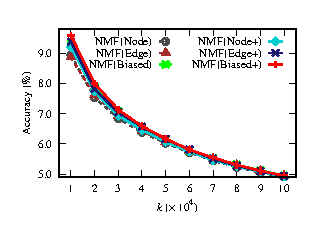
\includegraphics[width= 1.8in, height=1.2in]{eps-script/1-1-a.eps} }
  \quad\quad
  \subfigure[YouTube]{\label{fig_exp_1_1_k_acc_youtube}\includegraphics[width= 1.8in, height=1.2in]{eps-script/1-1-b.eps} }
  \quad\quad
  \subfigure[Wikipedia]{\label{fig_exp_1_1_k_acc_wikipedia}\includegraphics[width= 1.8in, height=1.2in]{eps-script/1-1-c.eps} }
  \subfigure[Digg]{\label{fig_exp_1_1_k_time_digg}\includegraphics[width= 1.8in, height=1.2in]{eps-script/1-1-e.eps} }
  \quad\quad
  \subfigure[YouTube]{\label{fig_exp_1_1_k_time_youtube}\includegraphics[width= 1.8in, height=1.2in]{eps-script/1-1-f.eps} }
  \quad\quad
  \subfigure[Wikipedia]{\label{fig_exp_1_1_k_time_wikipedia}\includegraphics[width= 1.8in, height=1.2in]{eps-script/1-1-g.eps}}
  \vspace{-1ex}
  \caption{Accuracy and efficiency comparison: with respect to the number $k$ of predicted links.}\label{fig_exp_1_1}
  \vspace{-2ex}
\end{figure*}

\begin{figure*}[tb!]
  \centering
  %\vspace{-2ex}
  % Requires \usepackage{graphicx}
  \subfigure[Digg]{\label{fig_exp_2_1_k_acc_digg}\includegraphics[width= 1.8in, height=1.2in]{eps-script/2-1-a.eps} }
  \hspace{-3ex}
  \subfigure[YouTube]{\label{fig_exp_2_1_k_acc_youtube}\includegraphics[width= 1.8in, height=1.2in]{eps-script/2-1-b.eps} }
  \hspace{-3ex}
  \subfigure[Wikipedia]{\label{fig_exp_2_1_k_acc_wikipedia}\includegraphics[width= 1.8in, height=1.2in]{eps-script/2-1-c.eps} }
  \hspace{-3ex}
  \subfigure[Flickr]{\label{fig_exp_2_1_k_acc_flickr}\includegraphics[width= 1.8in, height=1.2in]{eps-script/2-1-d.eps} }
  \subfigure[Digg]{\label{fig_exp_2_1_k_time_digg}\includegraphics[width= 1.8in, height=1.2in]{eps-script/2-1-e.eps} }
  \hspace{-3ex}
  \subfigure[YouTube]{\label{fig_exp_2_1_k_time_youtube}\includegraphics[width= 1.8in, height=1.2in]{eps-script/2-1-f.eps} }
  \hspace{-3ex}
  \subfigure[Wikipedia]{\label{fig_exp_2_1_k_time_wikipedia}\includegraphics[width= 1.8in, height=1.2in]{eps-script/2-1-g.eps}}
  \hspace{-3ex}
  \subfigure[Flickr]{\label{fig_exp_2_1_k_time_flickr}\includegraphics[width= 1.8in, height=1.2in]{eps-script/2-1-h.eps}}
  \vspace{-1ex}
  \caption{Accuracy and efficiency comparison: with respect to the number $k$ of predicted links.}\label{fig_exp_2_1}
  \vspace{-2ex}
\end{figure*}



\subsection{Comparison with \Aa, \RA and \BIGCLAM}
In this set of tests, we evaluated the robustness and efficiency of \Biased and \Biasedp
compared with \Aa, \RA and \BIGCLAM. We fixed $k$ to the number of links
in the ground truth data \cite{yang2015}, $r = 30$ on \Digg and \YouTube, $r = 20$ on \Wikipedia
and other parameters to their default values.
The results of accuracy together with their 95\% confidence intervals are reported
in Table \ref{tab_accuracy} and the results of running time are reported in Table \ref{tab_time}.

The accuracy results tell us that (a) \Biased and \Biasedp outperform other methods on
most of the datasets, (b) the accuracy of \Biasedp is very close to that of \Biased, (c) both
\Biased and \Biasedp have a higher accuracy than \NMF, \Aa, \RA and \BIGCLAM, except for \Aa and \RA on \Wikipedia,
and (d) \NMF is more accurate than \Aa, \RA and \BIGCLAM, except for \Aa and \RA on \Wikipedia.
Indeed, \Biased improves the accuracy by $(2.8\%, 24.3\%, 70.8\%, 11.9\%)$ (\resp $(1.5\%, 34.0\%, 34.0\%, 22.9\%)$
and $(11.0\%, -16.0\%, -51.3\%, 12.9\%)$) over \NMF, \Aa, \RA and \BIGCLAM on \Digg, \YouTube and \Wikipedia,
respectively. Moreover, \Biased and \Biasedp perform consistently well on all networks (\ie more robust), unlike \RA which works well
on \Wikipedia but poorly on other datasets. This verifies the robustness of our bagging methods.


The running time results tell us that (a) \Biasedp is the fastest among
\Biased, \NMF and \BIGCLAM, (b) the two bagging methods are much faster than \NMF and \BIGCLAM,
(c) the running time of \Aa and \RA increases rapidly with the increase of the network degree
 since their complexities are $O(nd^2\log(k))$.
Indeed, the bagging+ and bagging methods finished the prediction in 421 seconds on the three datasets.
Furthermore, \Biasedp is $(7.5, 0.2, 0.1, 1.2)$ (\resp $(8.8, 0.1, 0.1, 1.5)$ and $(11.4, 7.3, 6.1, 16.0)$)
times faster than \NMF, \Aa, \RA and \BIGCLAM on
\Digg, \YouTube and \Wikipedia, respectively.
This verifies the efficiency of our bagging methods.

\begin{table}
\caption{Accuracy (\%) comparison with \Aa, \RA and \BIGCLAM.}
\label{tab_accuracy}
\vspace{-2ex}
\centering
\newcommand{\tabincell}[2]{\begin{tabular}{@{}#1@{}}#2\end{tabular}}
\begin{tabular}{l|c|c|c}
\hline \hline Algorithm  & Digg & YouTube & Wikipedia  \\
\hline \hline
\Aa & 2.35 &	1.00 &	1.56  \\
\RA & 1.71 &	1.00 &	\textbf{2.69}  \\
\BIGCLAM & 2.61 $\pm$ (0.101) &	1.09 $\pm$ (0.107) &	1.16 $\pm$ (0.018)  \\
\NMF & 2.84 $\pm$ (0.056)	& 1.32 $\pm$ (0.059) 	& 1.18 $\pm$ (0.070) \\
\Biased & \textbf{2.92 $\pm$ (0.020)}	& 1.34 $\pm$ (0.059)	& 1.31 $\pm$ (0.018)\\
\Biasedp & 2.88 $\pm$ (0.054)	& \textbf{1.34 $\pm$ (0.044)}	& 1.30 $\pm$ (0.016) \\
\hline \hline
\end{tabular}
\vspace{-2ex}
\end{table}

\begin{table}
\caption{Running time (sec.) comparison with \Aa, \RA and \BIGCLAM.}
\label{tab_time}
\vspace{-2ex}
\centering
\newcommand{\tabincell}[2]{\begin{tabular}{@{}#1@{}}#2\end{tabular}}
\begin{tabular}{l|r|r|r}
\hline \hline Algorithm  & Digg & YouTube & Wikipedia  \\
\hline \hline
\Aa & 10.46 &	56.78 &	2557.63  \\
\RA & \textbf{7.74} &	\textbf{39.12} &	2136.36  \\
\BIGCLAM & 70.34 &	598.06 &	5642.84  \\
\NMF & 441.81 	& 3500.68 	& 4038.13 \\
\Biased & 64.58	& 420.21	& 393.26 \\
\Biasedp & 58.91	& 399.84	& \textbf{352.76} \\
\hline \hline
\end{tabular}
\vspace{-2ex}
\end{table}





\section{Appendix B Ensemble-Enabled Approach with AA and RA}

One interesting thing should be noted that our ensemble-enabled
approach is not only designed for \NMF, but also applied to any link
prediction methods. Therefore, we implemented \AABiased and \AABiasedp
(\resp \RABiased and \RABiasedp) by replacing \NMF with \Aa (\resp \RA) in
\Biased and \Biasedp. Furthermore, we evaluated the robustness and efficiency
of the ensemble-enabled approach with \Aa and \RA.
We varied $k$ from hundreds to the number of links in the ground truth data
and fixed other parameters to their default values. The results of accuracy
and running time are reported in Figures \ref{fig_exp_2_1_k_acc_digg}--\ref{fig_exp_2_1_k_acc_flickr}
and Figures \ref{fig_exp_2_1_k_time_digg}--\ref{fig_exp_2_1_k_time_flickr}, respectively.

The results of accuracy tell us that (a) \AABiased and \AABiasedp (\resp \RABiased and \RABiasedp)
are more accurate than \Aa (\resp \RA) on most of the datasets,
(b) the accuracy of \AABiasedp (\resp \RABiasedp) is close to that of \AABiased (\resp \RABiased).
This is verifies the robustness of the ensemble-enabled approach.

Note that \AABiased and \AABiasedp (\resp \RABiasedp)
perform worse than their counterpart \Aa (\resp \RA) on \Wikipedia because their diversities
on this dataset are poor. For instance, the pairwise overlapping of predicted links of \AABiased
(\resp \AABiasedp and \RABiasedp) is 0.62 (\resp 0.63 and 0.52). One reason for the decreasing
of diversity may be that the dataset contains some extreme high degree nodes,
\ie nodes with degree between $5 \times 10^4$ to $1.8 \times 10^5$.

The results of running time tell us that \AABiased and \AABiasedp (\resp \RABiased and \RABiasedp)
are faster than \Aa (\resp \RA) on \YouTube and \Wikipedia but
slower on other datasets. This is consistent with the complexity analysis
that the ensemble-enabled \Aa and \RA require $O(nd_{1}^{2}\log(k)\mu/f)$ time,
where $d_1$ is the average degree of each ensemble component. It is means
that the ensemble-enabled \Aa and \RA would be faster when $d_1$ is small.
Indeed, $d_1$ of \AABiased is 9 and 56 on \YouTube and \Wikipedia while the average
degree of these datasets is 5 and 33 respectively. However, $d_1$ of \AABiased is 30 and 75
on \Digg and \Flickr while the average degree of these datasets is 10 and 17 respectively.
The speedup of \AABiased and \AABiasedp (\resp \RABiased and \RABiasedp) are (5, xx) and (14, xx) 
(\resp (7, xx) and (20, xx)) on the large networks \Twitter and \Friendster, which verifies the efficiency 
of our ensemble-enabled approach.





\begin{footnotesize}
\bibliographystyle{abbrv}
\bibliography{paper}
\end{footnotesize}

%\begin{table}
%\caption{Accuracy (\%) comparison with \Aa, \RA and \BIGCLAM.}
%\label{tab_accuracy2}
%\vspace{-2ex}
%\centering
%\newcommand{\tabincell}[2]{\begin{tabular}{@{}#1@{}}#2\end{tabular}}
%\begin{tabular}{l|c|c|c}
%\hline \hline Algorithm  & Digg & YouTube & Wikipedia  \\
%\hline \hline
%\Aa & 2.35 &	1.00 &	1.56  \\
%\RA & 1.71 &	1.00 &	\textbf{2.69}  \\
%\BIGCLAM & 2.61 $\pm$ (0.101) &	1.09 $\pm$ (0.107) &	1.16 $\pm$ (0.018)  \\
%\NMF & \textbf{2.86 $\pm$ (0.082)}	& \textbf{1.33 $\pm$ (0.087)} 	& 1.19 $\pm$ (0.047) \\
%\hline
%\Node & 2.92 $\pm$ (0.017)	& 1.35 $\pm$ (0.086)	& 1.29 $\pm$ (0.026) \\
%\Edge & \textbf{2.93 $\pm$ (0.029)}	& \textbf{1.35 $\pm$ (0.065)}	& 1.31 $\pm$ (0.023) \\
%\Biased & 2.92 $\pm$ (0.020)	& 1.34 $\pm$ (0.059)	& \textbf{1.31 $\pm$ (0.018) }\\
%\hline
%\Nodep & 2.86 $\pm$ (0.020)	& 1.36 $\pm$ (0.040)	& 1.30 $\pm$ (0.031) \\
%\Edgep & \textbf{2.90 $\pm$ (0.032)}	& \textbf{1.38 $\pm$ (0.041)}	& 1.30 $\pm$ (0.012) \\
%\Biasedp & 2.88 $\pm$ (0.054)	& 1.37 $\pm$ (0.062)	& \textbf{1.32 $\pm$ (0.022)} \\
%\hline \hline
%\end{tabular}
%\vspace{-2ex}
%\end{table}
%
%\begin{table}
%\caption{Running time (sec.) comparison with \Aa, \RA and \BIGCLAM.}
%\label{tab_time2}
%\vspace{-2ex}
%\centering
%\newcommand{\tabincell}[2]{\begin{tabular}{@{}#1@{}}#2\end{tabular}}
%\begin{tabular}{l|r|r|r}
%\hline \hline Algorithm  & Digg & YouTube & Wikipedia  \\
%\hline \hline
%\Aa & 10.46 &	56.78 &	2557.63  \\
%\RA & 7.74 &	39.12 &	2136.36  \\
%\BIGCLAM & 70.34 &	598.06 &	5642.84  \\
%\NMF & 417.33 	& 3695.67 	& 4690.71 \\
%\hline
%\Node & 74.62	& 431.52	& 403.51 \\
%\Edge & 78.76	& 446.22	& 410.86 \\
%\Biased & 64.58	& 420.21	& 393.26 \\
%\hline
%\Nodep & 65.95	& 405.29	& 356.77 \\
%\Edgep & 68.26	& 415.26	& 374.73 \\
%\Biasedp & 58.91	& 399.84	& 353.12 \\
%\hline \hline
%\end{tabular}
%\vspace{-2ex}
%\end{table}


\end{document}
